\documentclass{article}
\usepackage{enumerate}
\usepackage{titling}
\usepackage{fullpage}
\usepackage{amsmath}
\usepackage{amsfonts}
\usepackage{amsthm}
\usepackage{float}
\usepackage{stmaryrd}
\usepackage{graphicx}
\usepackage{caption}
\usepackage{subcaption}
\usepackage{color}
\usepackage{multicol}
\usepackage{wrapfig}
\usepackage{enumitem}
\usepackage[labelfont=bf]{caption}
\usepackage{mdframed}
\usepackage{framed}
\usepackage{hyperref}

\hypersetup{
    colorlinks=true,
    linkcolor=blue,
    filecolor=blue,
    urlcolor=blue,
}

\urlstyle{same}

\graphicspath{ {C:/Users/notle_000/Documents/NYC_Transportation_Weather_Study/Visuals/} }

\title{CSCI 6350 Data Science Assignment 4: Examining the Effects of Weather on Taxi Service in New York City}

\author{Stephen Notley, Diana Edwards, Ian Gross, Jianhui Lu, \& Animesh Tripathy}
\date{12/1/2017}
\setlength{\droptitle}{-1in}

\begin{document}
\maketitle

\begin{enumerate}

    \item %PART 1

    The team chose to examine the relationship between weather and taxi usage statistics in New York City in order to better understand how weather effects taxi service demand and performance. The specific questions posed will be elaborated on in greater detail in Part 2 below.

    \begin{enumerate}

        \item %PART 1-a
        The team chose the 2016 Taxi data because of its convenient and detailed information about pickup and dropoff times, distances, number of passengers, and trip duration in seconds, which will allow for many interesting relationships to be explored. This data was sourced from the NYC TLC, the page for which can be found \href{http://www.nyc.gov/html/tlc/html/about/trip_record_data.shtml}{\underline{here}}. After briefly exploring a condensed version of the yellow line data found in a Kaggle competition (found \href{https://www.kaggle.com/c/nyc-taxi-trip-duration/data}{\underline{here}}) and finding no statistically-relevant correlations between this data and various statistics, the team decided to focus on the green line data, as stronger correlations were found here for reasons that will be discussed later.

        The weather data was sourced from Weather Underground (page found \href{https://www.wunderground.com/history/airport/KJFK/2016/1/2/MonthlyHistory.html?&reqdb.zip=&reqdb.magic=&reqdb.wmo=}{\underline{here}}), which has historical weather data available for New York City, measured at JFK International Airport, which contains daily metrics of temperature, wind speed, visibility, and conditions, among other stats. This was obtained by use of a scraping tool to gather the data from the monthly pages throughout 2016.

        The size of the green line taxi data is rather large (~2GB) and so was stored on a Google Drive (\href{https://drive.google.com/file/d/1wPVIqUaaxgLZLQ8ahNiXleMFAO_wE2b2/view?usp=sharing}{\underline{here}}), while the weather data can be found on the GitHub page for the project \href{https://github.com/IanGross/NYC_Transportation_Weather_Study}{\underline{here}}. %FILENAME

        \item %PART 1-b
        The Kaggle Yellow line taxi data came in a zipped csv file, with each row representing one trip and each column representing various statistics about each trip. The metadata here was simply a plain text pairing system of column title and an explanation of what it meant in plain English with units. The Green line data is from the NYC Taxi and Limousine Commission, Trip Record Data page. Each trip sheet data is stored by Year, Month, and the taxi line (Yellow, Green or FHV) in the form of a csv file. Data dictionary pdfs provide a description for each dataset's Field Name.
		The weather data was available on a web page (Weather Underground historical KJFK page), from which a script was used to scrape the JavaScript into a csv file, which was labeled with appropriate column names as metadata. The only additional piece of metadata collected on the weather data was the location of its collection: JFK International Airport. 
		The team also decided to aggregate the unwieldy individual taxi trip data into a statistics csv file, which consisted of a datapoint for each day, giving the total number of taxi passengers that day, the average number of passengers per ride, the number of rides, the average disance and speed of rides, and average trip duration. The team thought that these aggregated statistics could be used to see meaningful correlations during analysis. Metadata for these statistics can be found in the metadata.json file found on the GitHub page.


    \end{enumerate}

    \item %PART 2
    \begin{enumerate}

        \item %PART 2-a

        The two questions that the group hoped to answer using these datasets were:

        \begin{enumerate}
            \item
            How do various weather conditions affect taxi trip durations in New York City?

            \item
            How do various weather conditions affect the amount of people using taxis in New York City?

        \end{enumerate}

        The data analysis started with locating the data for weather data as well as taxi data which had, at minimum, details on duration, distance, and number of passengers (after aggregation). The weather data was scraped off of the Weather Underground website into a CSV file where it was then curated by month. Correlations and graphs were produced in order to determine any effects on the number of rides/passengers or trip duration. The statistics aggregated from the Kaggle yellow-line taxi data showed no statistically-significant correlations to the weather data, and so the team decided to halt the analysis on the yellow line at this point. The team hypothesized that this was because the yellow line primarily services manhattan, where traffic is too congested for weather to have much effect on duration. The green line, however, which runs outside of Manhattan, displayed several statisically-significant correlations with the weather data and contained a larger sample size.


        \item %PART 2-b

        An extension in Google Chrome called Data Miner was used to scrape data generated for 2016 from the Weather Underground website's JFK International Airport histroical data page. Data was scraped into a CSV file in order to be edited to a suitable format with appropriate column names. Additionally, duplcate column headers were removed and a month column was added manually in excel. Data was gathered from Kaggle and the TLC NYC taxi data page respectively. Due to TLC data was separated by month, a python script combined these files and removed unecessary columns. A C++ program was used to distill aggregated statistics from the taxi data to the statistics.csv file, which contained averaged/aggregated stats for each day in 2016. A Python script was used to create a heatmap (with the Python visualization library: Seaborn) which showed correlations between the computed daily taxi statistics and weather conditions to decide what was significant enough to warrant further analysis. This further analysis was performed using another python script with the matplotlib package. The script provided visualizations in the form of bar charts and scatter plots.
		Kaggle was used to obtain a condensed version of the New York City yellow line taxi transportation data. The original green line data was managed and stored in a shared Google Drive because of the size of the file. The results of the overall project and graphs were stored and managed in folders on Github. Each new result was pushed to the master branch and reviewed by the team. All scripts mentioned can be found in the scripts folder of the GitHub. Descriptions of these scripts are provided in the metadata document of the Github repository.


        \item %PART 2-c

        The steps taken to perform the analysis were locating the data relevant to our study, parsing through all the data, splitting up the data, separating the data from the metadata (which is included in a JSON file) and then conducting analysis on the data by using scripts to produce graphs displaying relationships pertinent to the questions posed. After the data was obtained, it had to be reformatted into a fashion that facilitated analysis to answer the questions posed by the team. The team wrote scripts to validate the analysis by reasoning about real-world phenomena in accordance with the results of the study.

    \end{enumerate}

    \item %PART 3
    \begin{enumerate}

        \item %PART 3-a

        Included below are the visualizations that the team found interesting, all visualizations created can be found in the Visuals folder on the project GitHub page.

        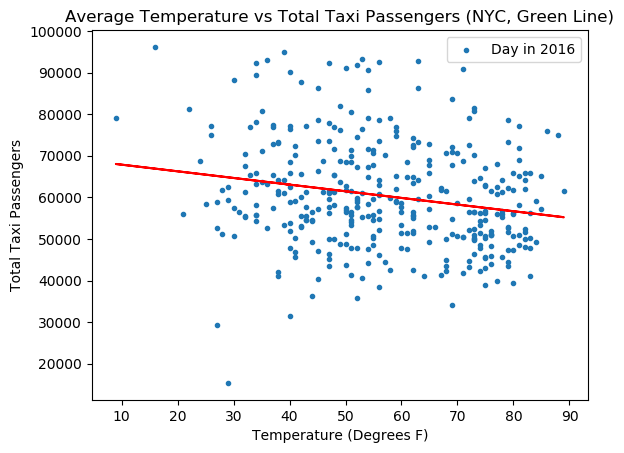
\includegraphics[width=7cm,height=5.25cm]{Scatter_Plots/Average_Temperature/Average_Temperature_vs_Total_Taxi_Passengers}
        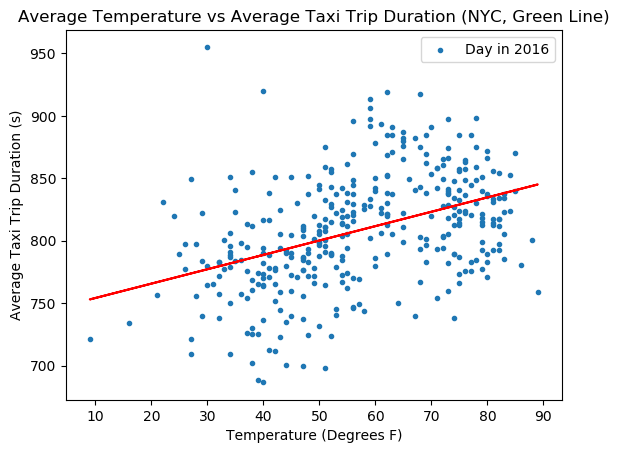
\includegraphics[width=7cm,height=5.25cm]{Scatter_Plots/Average_Temperature/Average_Temperature_vs_Average_Taxi_Trip_Duration}
        
        These two images paint a very picture in relation to our questions, showing that more people tend to take taxis when the temperature is lower, but that temperature has a minimal effect on trip duration (only a few minutes difference on average).
        
        \begin{center}
            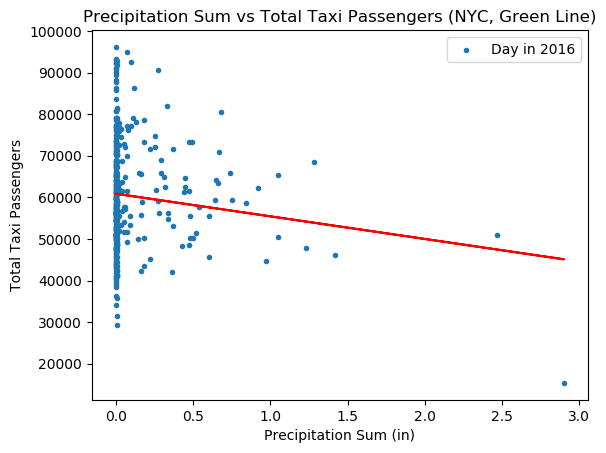
\includegraphics[width=7cm,height=5.25cm]{Scatter_Plots/Precipitation_Sum/Precipitation_Sum_vs_Total_Taxi_Passengers}
        \end{center}
        
        This correlation suggests that far less people take taxis when there is a significant amount of precipitation, likely because people prefer not to travel around the city at all in inclement weather, if avoidable.
        
        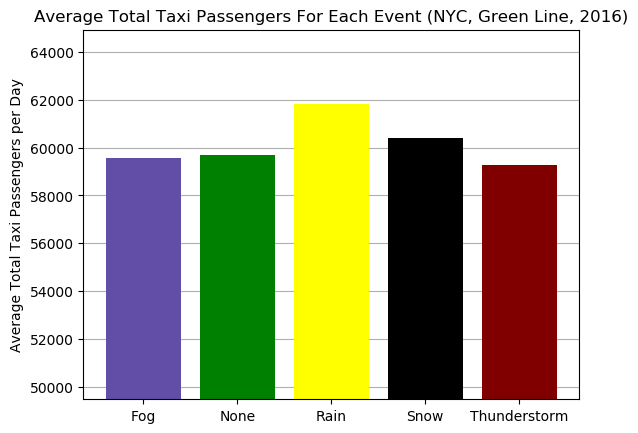
\includegraphics[width=7cm,height=5.25cm]{Event_Bar_Charts/Event_Bar_Chart_Average_Total_Taxi_Passengers}
        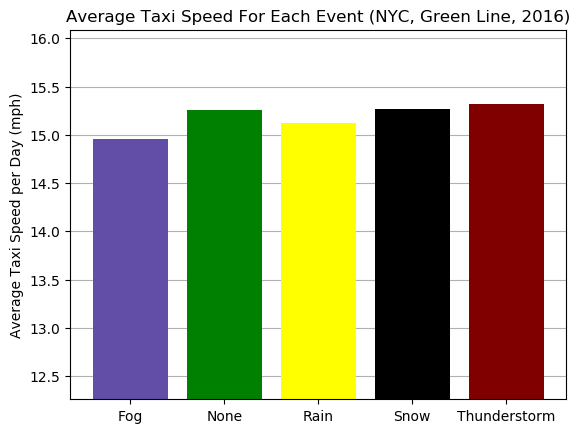
\includegraphics[width=7cm,height=5.25cm]{Event_Bar_Charts/Event_Bar_Chart_Average_Taxi_Speed}
        
        In terms of weather events, the above visuals show that the most passengers tend to use taxi services on rainy days and that foggy days cause the most decrease in speed, both of which intuitively make sense. That being said, neither makes a particularly striking difference.
        
        Overall, after analyzing the trends in the data the conclusion is that inclement weather, particularly cold and rain, cause more people to take taxis in New York City, although the impact is less than expected. Even further from what the team predicted, inclement weather has a very minimal effect on the speed of taxi trips. Upon further consideration, the team realizes that, although there is more room for effect than in the Manhattan-based yellow line data, average speeds are still low for this data, which means that weather likely would not have as much impact as on roads with higher speeds such as highways.

        \item %PART 3-b
        The visualizations are available on the GitHub page in the Visuals folder. The metadata associated with each visual is located in the title, x and y axis label, and the legend. This information describes the time of each data point, location (physical and source) and units.

        \item %PART 3-c
        These visualizations demonstrate the relationships between weather and taxi trip duration/speed as well as the number of people using taxis in these varying weather conditions, as was the goal of this study. The team concludes that inclement weather causes slightly more taxi usage but very minimal, if any, difference in taxi speed and trip duration. Although this result is counterintuitive, that is the very reason that it adds value- weather delay calculations are often a big part of travel logistics calculations and, this study shows that, at least for taxis in New York City, it may not need to be. This information, therefore, could potentially be quite useful in business logistics and planning in terms of taxi companies.


    \end{enumerate}

    \item %PART 4

    \begin{enumerate}

        \item
        \textbf{Logical Collections:}

        All datasets are named according to their corresponding data source. The columns of each dataset are named to accurately represent the given field, with units included in the name where applicable. Each row represents one day's worth of aggregate data for the weather and statistics files, while in the raw taxi data each row represents an individual taxi trip.


        \item
        \textbf{Physical Data Handling:}

        There were two datasets that were utilized for the transportation weather study. NYC Green Line taxi dataset was acquired from the NYC Taxi and Limousine Commission. Due to the Green Line taxi data being stored by month, it needed to be combined into a single 2016 file using a python script. The resulting combined dataset was processed through a C++ script named condense.cpp, which provided an aggregated statistics file. Weather data near JFK Airport for 2016 was exported from The Weather Company’s Wunderground application and reformatted to accommodate for the header structure of each month. Both datasets were processed and archived in comma separated value (CSV) file formats with their appropriate dataset names.


        \item
        \textbf{Interoperability Support:}

        The files containing each individual dataset were stored in close proximity using hierarchical file-folder layout to enable interoperability. All scripts, python notebooks, and python files could access the appropriate dataset files with ease due to standardized naming conventions and single storage location within a GitHub repository. Furthermore, all scripts and data files are encoded in a generic format that should be accessible on a wide variety of software and hardware media.


        \item
        \textbf{Security:}

        Datasets were managed and maintained by outside vendors, more specifically, NYC TLC and The Weather Company. Data is secured and changed on the NYC government and IBM servers, respectively. Data were acquired through an export tool which was processed and stored in a secured GitHub repository. Access to processed data can only be attained by authorized Group 5 members via their GitHub accounts.


        \item
        \textbf{Data Ownership:}

        NYC TLC data has strictly noted that their data collected is not used, sold, or exchanged for commercial or marketing purposes. Data is automatically collected and quality assured by the NYC government. The Weather Company is operated under IBM with little to no restrictions on access to their data. Data is automatically collected and quality managed from weather devices and applications used by IBM.


        \item
        \textbf{Metadata:}

        Metadata for each dataset were noted within the file labeled metadata.json. Each file was provided a description identifying where the data was obtained from and what processes had been taken to refine them and a fields section noting the column names and appropriate definitions.


        \item
        \textbf{Persistence:}

        Raw datasets for both NYC TLC and Wunderground are found on their respective websites noted in the metadata. The processed versions of each dataset is published on the NYC Transportation Weather Study GitHub public repository hosted by Ian Gross. Due to the file size of the Green Line Taxi data, it is accessible on Ian Gross's Google Drive via a link provided earlier in the document.


        \item
        \textbf{Discovery:}

        The processed datasets can be found via the NYC Transportation Weather Study GitHub public repository to enable outsiders to gain access to each dataset. Anyone who desires can request access to this from Ian Gross who manages the repository. This also applies to the aggregate Green line taxi data stored on his Google Drive.


        \item
        \textbf{Dissemination:}

        A project description and appropriate topics will be provided to create connections between interested parties and our datasets. GitHub allows for all changes and additions to be publicized to all outside parties and enables them to track via GitHub issues. GitHub enables the team to disseminate and connect external users to our data project management.
        
    
    \end{enumerate}



\end{enumerate}


\end{document} 